\chapter{Design and Implementation} \label{sec:DI}

This chapter will discuss, in detail, the methods used and the approaches taken when implementing solutions to the two primary tasks this dissertation is concerned with: the prediction of various review features using only the review text and the identification of users who best represent the population of reviewers, as a whole, through the content of their written reviews.

\section{Review Feature Prediction} \label{sec:DI_RF}

In this section, the process of selecting and training optimal machine learning models with the goal of predicting three features of a given review will be discussed. The review features being predicted are: its polarity, how many helpfulness votes it received and the length of time the reviewer spent playing the game. The machine learning models that will be tested are BERT, specifically two pretrained DistilBERT models; MNB and CNB classifiers; linear SVMs for classification and regression, both with SGD and without; a ridge regressor; and multiple baseline classifiers and regressors.

\subsection{Dataset Sampling} \label{sec:DI_RF_Sampling}

Due to the time and memory-consuming nature of the model training procedure in machine learning, especially when considering neural networks like BERT, it would be unfeasible to utilise the entirety of the dataset, which consists of over 10 million reviews, in the model training and testing processes. Instead, numerous samples of the dataset, each containing exactly 100 thousand reviews, were prepared and used to train the predictive models.

Only reviews consisting of at least one word, determined by the process outlined in section \ref{sec:Dataset_RT_Langs}, were included when preparing the dataset samples. The language that a review was written in was considered a determining factor in relation to how well the trained models would be able to accurately predict the selected review features. As such, separate samples were prepared for reviews written in English\footnote{Reviews that were classified as English with a confidence of at least 70\% by the language detection algorithm discussed in \ref{sec:Dataset_RT_Langs} were included in the English-language samples.} and reviews written in any language (including English). Also of interest was the potential effect that the length of the review text, ie the word count, might have on the accuracy of the trained models' predictions. As such, separate samples were prepared for reviews that contained 50 words or more, referred to as `long' reviews; reviews that contained fewer than 50 words, referred to as `short' reviews; and reviews containing any number of words.

Several samples were also prepared solely for the task of review polarity prediction. Due to the imbalanced nature of the dataset with regard to review polarity, 85\% of reviews are positive while only 15\% of reviews are negative, and, since this task is a classification problem, separate samples were prepared containing equal numbers of positive and negative reviews in order to more accurately determine how well the trained models were performing.

The names and characteristics of all of the prepared data samples are given in Table \ref{tab:DI_RF_Datasets}.

\begin{table}[ht]
    \centering
    \begin{tabular}{l|l l l l}
        \toprule
        \textbf{Sample Name} & \textbf{Language} & \textbf{Length} & \textbf{Balanced} & \textbf{Size}\\\midrule
        \texttt{eng\_eq\_any} & English & Any & Yes & 100k\\
        \texttt{eng\_eq\_short} & English & Short & Yes & 100k\\
        \texttt{eng\_eq\_long} & English & Long & Yes & 100k\\
        \texttt{any\_eq\_any} & Multilingual & Any & Yes & 100k\\
        \texttt{any\_eq\_short} & Multilingual & Short & Yes & 100k\\
        \texttt{any\_eq\_long} & Multilingual & Long & Yes & 100k\\
        \texttt{eng\_any\_any} & English & Any & No & 100k\\
        \texttt{eng\_any\_short} & English & Short & No & 100k\\
        \texttt{eng\_any\_long} & English & Long & No & 100k\\
        \texttt{any\_any\_any} & Multilingual & Any & No & 100k\\
        \texttt{any\_any\_short} & Multilingual & Short & No & 100k\\
        \texttt{any\_any\_long} & Multilingual & Long & No & 100k\\
        \bottomrule
    \end{tabular}
    \caption{Dataset samples and their characteristics for review feature prediction.}
    \label{tab:DI_RF_Datasets}
\end{table}

\subsection{Polarity} \label{sec:DI_RF_Pol}

\subsubsection{BERT}

\paragraph{Data Splitting}

Each dataset sample was split into three sets: training (80\% of the sample), validation (10\% of the sample) and test (10\% of the sample). The training set was used to fine-tune the BERT model, the validation set was used to evaluate the trained model after each epoch and the test set was used to determine the overall quality of the fully trained model.

\paragraph{Preprocessing}

Very little preprocessing needed to be done to the data before it was passed into the BERT model for training. Tokenisation was done using the pretrained tokenisers that were provided with both the English-language and multilingual DistilBERT models. The tokenised input data, alongside the output polarity data, were converted to tensors, before being used to fit the BERT classifier.

\paragraph{Hyperparameter Tuning}

Optimal training parameters were selected for all of the BERT models used to predict review polarity by testing numerous combinations of parameters on a model trained using the \texttt{eng\_eq\_any} sample. Individually applying the hyperparameter tuning process to each of the dataset samples, even if it may have led to slightly better results for those samples, would have been far too time-consuming to carry out.

The learning rate of the Adam optimiser, which is used by the classifier, was originally considered as a tunable parameter; however, experimenting with its value did not to lead to any improvements and, as such, it was not considered in the final approach. The two parameters which were settled on were the batch size and the number of epochs the model was to be trained for. The parameter values that were considered can be seen in Table \ref{tab:DI_RF_Pol_BERTHP}.

\begin{table}[ht]
    \centering
    \begin{tabular}{l l}
        \toprule
        \textbf{Hyperparameter} & \textbf{Values}\\\midrule
        Batch size & $16, 32, 64$\\
        Epochs & $2, 3, 4$\\
        \bottomrule\\
    \end{tabular}
    \caption{BERT hyperparameters for review polarity.}
    \label{tab:DI_RF_Pol_BERTHP}
\end{table}

The training and validation accuracies of the trained models for each combination of hyperparameters can be seen in Figure \ref{fig:DI_RF_Pol_BERTHP}.

\begin{figure}[ht]
    \centering
    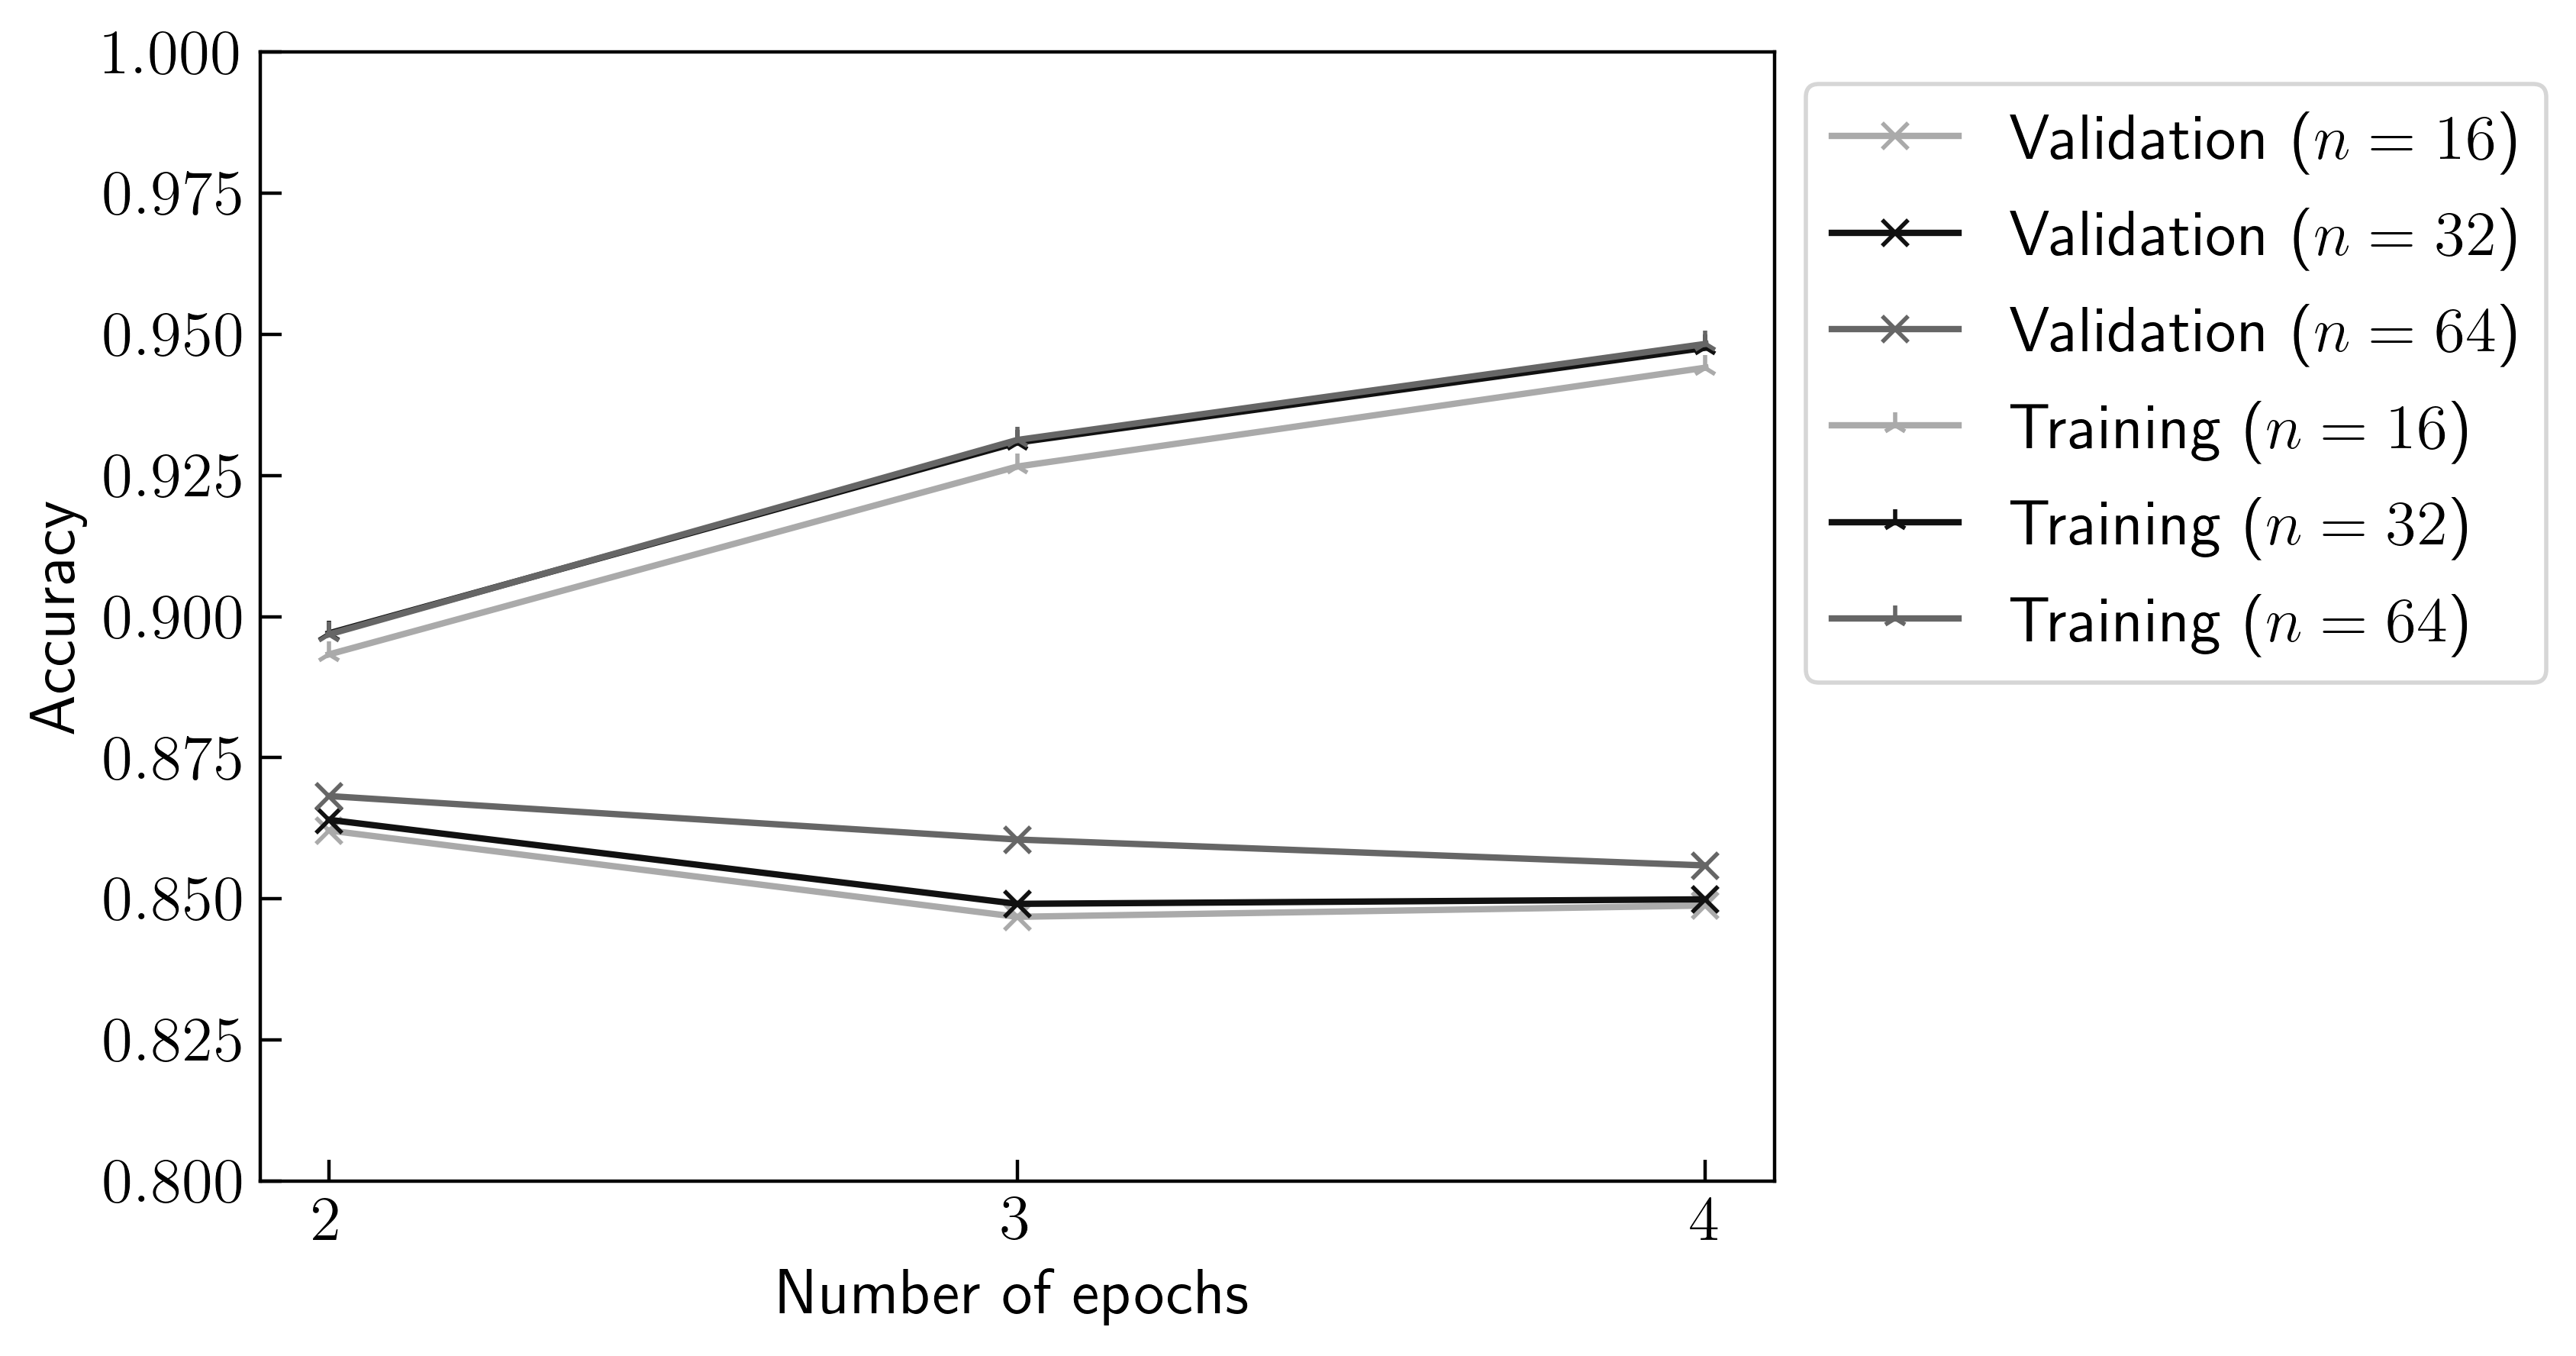
\includegraphics[scale=0.7]{figures/05_impl/01_rfp/01_pol/plot_hyperparams_bert.png}
    \caption{BERT hyperparameter tuning results for review polarity ($n$ is batch size).}
    \label{fig:DI_RF_Pol_BERTHP}
\end{figure}

Based on these results it is clear that the classifiers begin to overfit the training data after 2 epochs as the training accuracy begins to increase at the expense of the validation accuracy. The models trained with a batch size of 64 also appear to perform the strongest and, as such, the combination of 2 epochs and a batch size of 64 will be used when training and testing BERT models for the other dataset samples.

\paragraph{Training Procedure}

BERT models were trained and validated for all 12 dataset samples using the optimal hyperparameters. Samples containing English reviews were trained using the pretrained \texttt{distilbert-base-uncased} model while multilingual samples were trained using the \texttt{distilbert-base-multilingual-cased} model. Their performance was then tested using the test sets of their respective samples. The results of these tests will be discussed, in detail, in section \ref{sec:Res_RF_Pol}.

\subsubsection{Other Models}

\paragraph{Data Splitting}

In contrast to the procedure utilised when training BERT models, the dataset samples were split into two sets rather than three: training (90\% of the sample) and test (10\% of the sample). The training results were gathered using the mean accuracy of 5-fold cross-validation performed on the training set as opposed to the validation accuracy taken from the BERT training process. The test results were gathered in the same manner as the BERT test results were gathered.

\paragraph{Preprocessing}

Unlike with BERT, significant preprocessing needed to be applied to the review text data before it could be passed into a model for training. The steps involved in this process are as follows:

\begin{enumerate}
    \item Convert the text to lowercase\footnote{Only for English-language reviews.}.
    \item Replace all non-word characters\footnote{Any Unicode character that is not a letter used in words in any language.} with spaces.
    \item Split the text into words based on spaces.
    \item Remove any stopwords.
    \item Join the remaining words back together and remove repeated spaces.
    \item Vectorise the text.
    \item Apply TF-IDF weightings to the vectorised text.
\end{enumerate}

The text was also processed into various sets of $n$-grams before being used in model training; however, this process will be discussed in the following section. The list of stopwords used were provided by Python's NLTK library \cite{bird2009natural} which contains stopword lists for 24 different languages.

\paragraph{Hyperparameter Tuning}

As was the case with BERT, optimal hyperparameters for each model were selected based on the results gathered for the \texttt{eng\_eq\_any} sample due to the time-consuming nature of the training process.

Regardless of the model being used, the review text was converted into sets of $n$-grams of varying sizes and ranges\footnote{The $n$-gram range of $(1, 2)$, for example, would consist of all unigrams and bigrams taken from the text.}. For the MNB, CNB and SGD classifiers, the $\alpha$ parameter was varied. For the LSVC, the $C$ parameter was varied. Parameter ranges were chosen so as to provide a large amount of variance between results so that the optimal parameters for each model could be accurately selected. The parameter values that were considered can be seen in Table \ref{tab:DI_RF_Pol_BaseHP}.

\begin{table}[ht]
    \centering
    \begin{tabular}{l l l}
        \toprule
        \textbf{Model} & \textbf{Hyperparameter} & \textbf{Values}\\\midrule
        All & $n$-gram range & $(1, 2), (1, 3), (1, 4)$\\
        MNB & $\alpha$ & $0.01, 0.1, 1, 10$\\
        CNB & $\alpha$ & $0.01, 0.1, 1, 10$\\
        SGD & $\alpha$ & $10^{-4}, 10^{-5}, 10^{-6}$\\
        LSVC & $C$ & $0.01, 0.1, 1, 10$\\
        \bottomrule\\
    \end{tabular}
    \caption{Other model hyperparameters for review polarity.}
    \label{tab:DI_RF_Pol_BaseHP}
\end{table}

Two baseline classifiers were also used for comparison: one which predicted a random class and one which predicted the most frequent class. The mean cross-validation accuracies for each combination and model can be seen in Figure \ref{fig:DI_RF_Pol_BaseHP}. The standard deviations of the cross-validation accuracies were also gathered; however, they were all found to be insignificantly small and, as such, have not been included in the plot.

\begin{figure}[ht]
    \hspace*{-0.3in}
    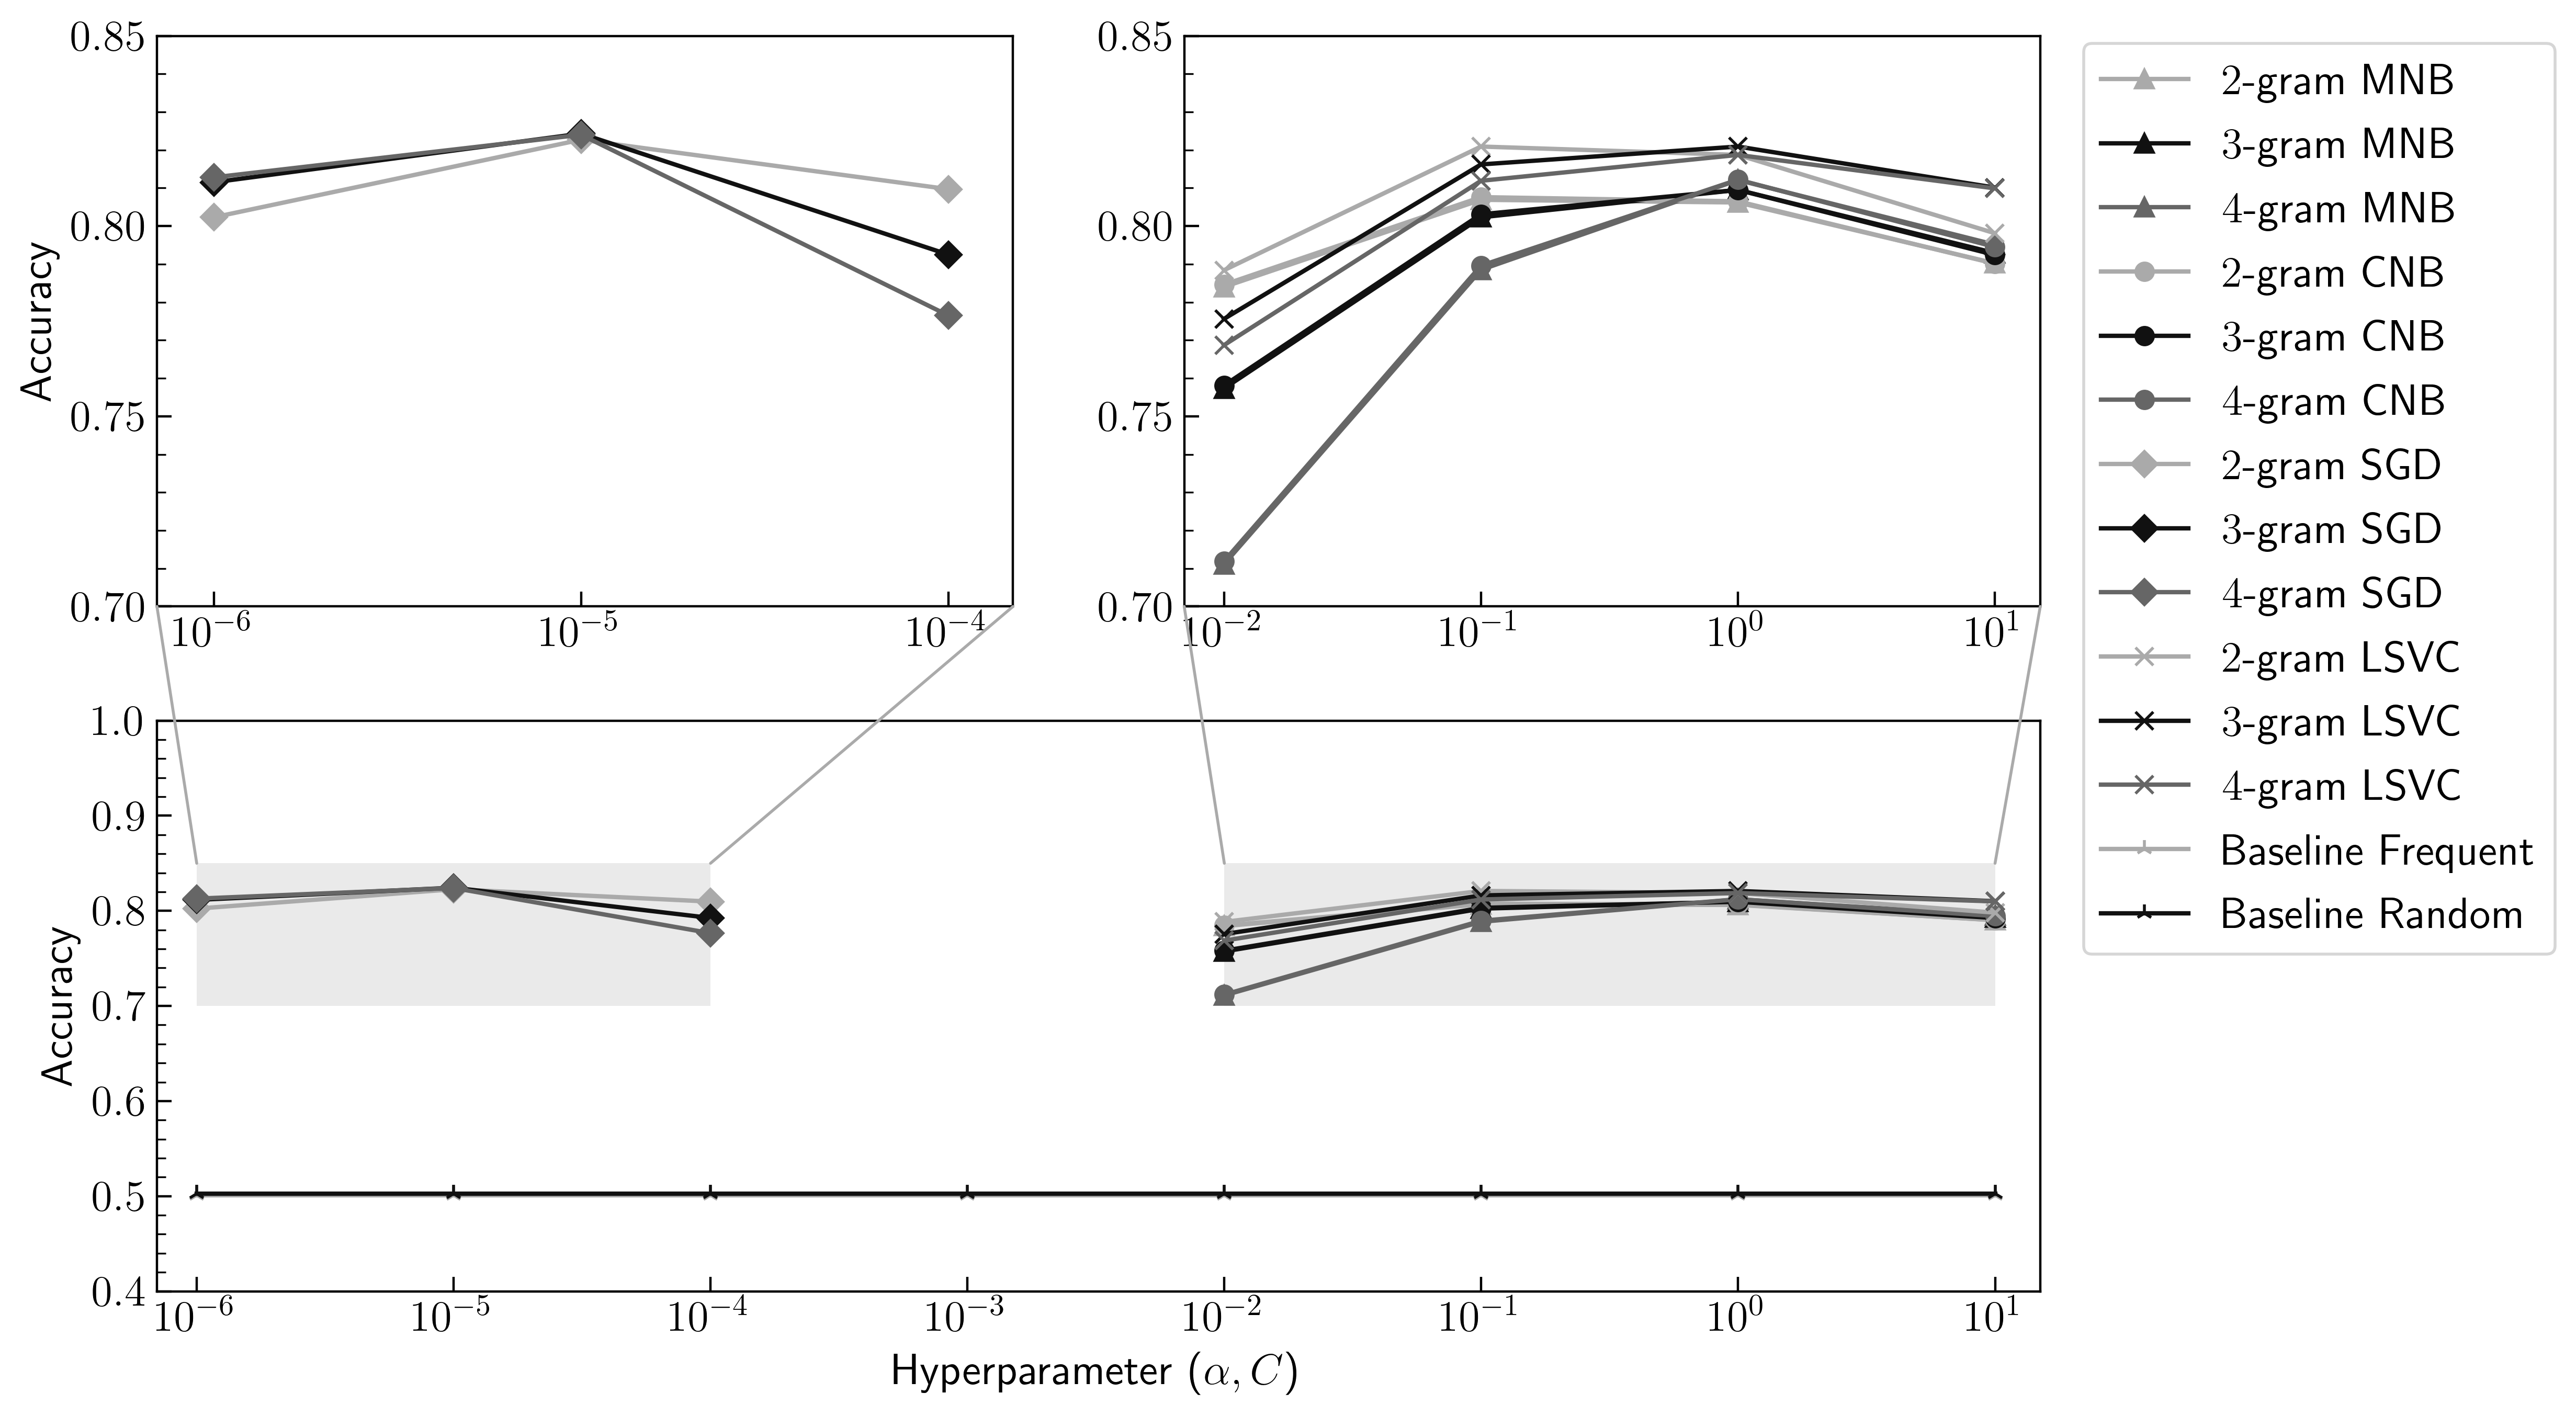
\includegraphics[scale=0.55]{figures/05_impl/01_rfp/01_pol/plot_hyperparams_base.png}
    \caption{Other model hyperparameter tuning results for review polarity.}
    \label{fig:DI_RF_Pol_BaseHP}
\end{figure}

Based on these results it seems that, for each SGD classifier, the parameter value of $\alpha=10^{-5}$ is optimal. The $n$-gram range of $(1, 3)$ also seems to have the best performance for that $\alpha$, though not by much. For the LSVC, a parameter value of $C=1$ with an $n$-gram range of $(1, 3)$ appears to be the best choice, although $C=0.1$ with an $n$-gram range of $(1, 2)$ performs almost as well.

Both of the NB classifiers seem to produce very similar results for each choice of $\alpha$ and $n$-gram range. In each case, it is clear that a parameter value of $\alpha=1$ with an $n$-gram range of $(1,4)$ is the best performing combination.

\paragraph{Training Procedure}

Each of the optimal classifiers was trained on all 12 dataset samples and their performance was then tested using the test sets of their respective samples. The test results will be discussed, and compared to the BERT results, in section \ref{sec:Res_RF_Pol}.

\subsection{Votes} \label{sec:DI_RF_Votes}

The process of training the machine learning models to predict the number of helpfulness votes that reviews received was very similar to the process used to predict their polarity. One key difference in the procedure was that the balanced dataset samples, ie those with 50\% positive and 50\% negative reviews, were not relevant to the task and were, as a result, not included.

\subsubsection{BERT}

\paragraph{Data Splitting}

The dataset samples were split into the same three sets, with the same proportions, that were mentioned for the BERT model in section \ref{sec:DI_RF_Pol}.

\paragraph{Preprocessing}

As was also discussed previously, very little preprocessing needed to be done to the text data before being passed into the BERT model. However, a robust scaler was used to map the number of votes each review received down to a limited range centered around 0. A robust scaler was used due to the presence of outliers in the dataset.

\paragraph{Hyperparameter Tuning}

Optimal training parameters were selected for all of the BERT models based on the results gathered for the \texttt{eng\_any\_any} sample. The same combinations of batch size and training epochs were tested for the prediction of review votes as were tested for the prediction of review polarity. These values can be seen, again, in Table \ref{tab:DI_RF_Votes_BERTHP}.

\begin{table}[ht]
    \centering
    \begin{tabular}{l l}
        \toprule
        \textbf{Hyperparameter} & \textbf{Values}\\\midrule
        Batch size & $16, 32, 64$\\
        Epochs & $2, 3, 4$\\
        \bottomrule\\
    \end{tabular}
    \caption{BERT hyperparameters for review votes.}
    \label{tab:DI_RF_Votes_BERTHP}
\end{table}

The NMSE loss for both the training and validation sets can be seen in Figure \ref{fig:DI_RF_Votes_BERTHP}.

\begin{figure}[ht]
    \centering
    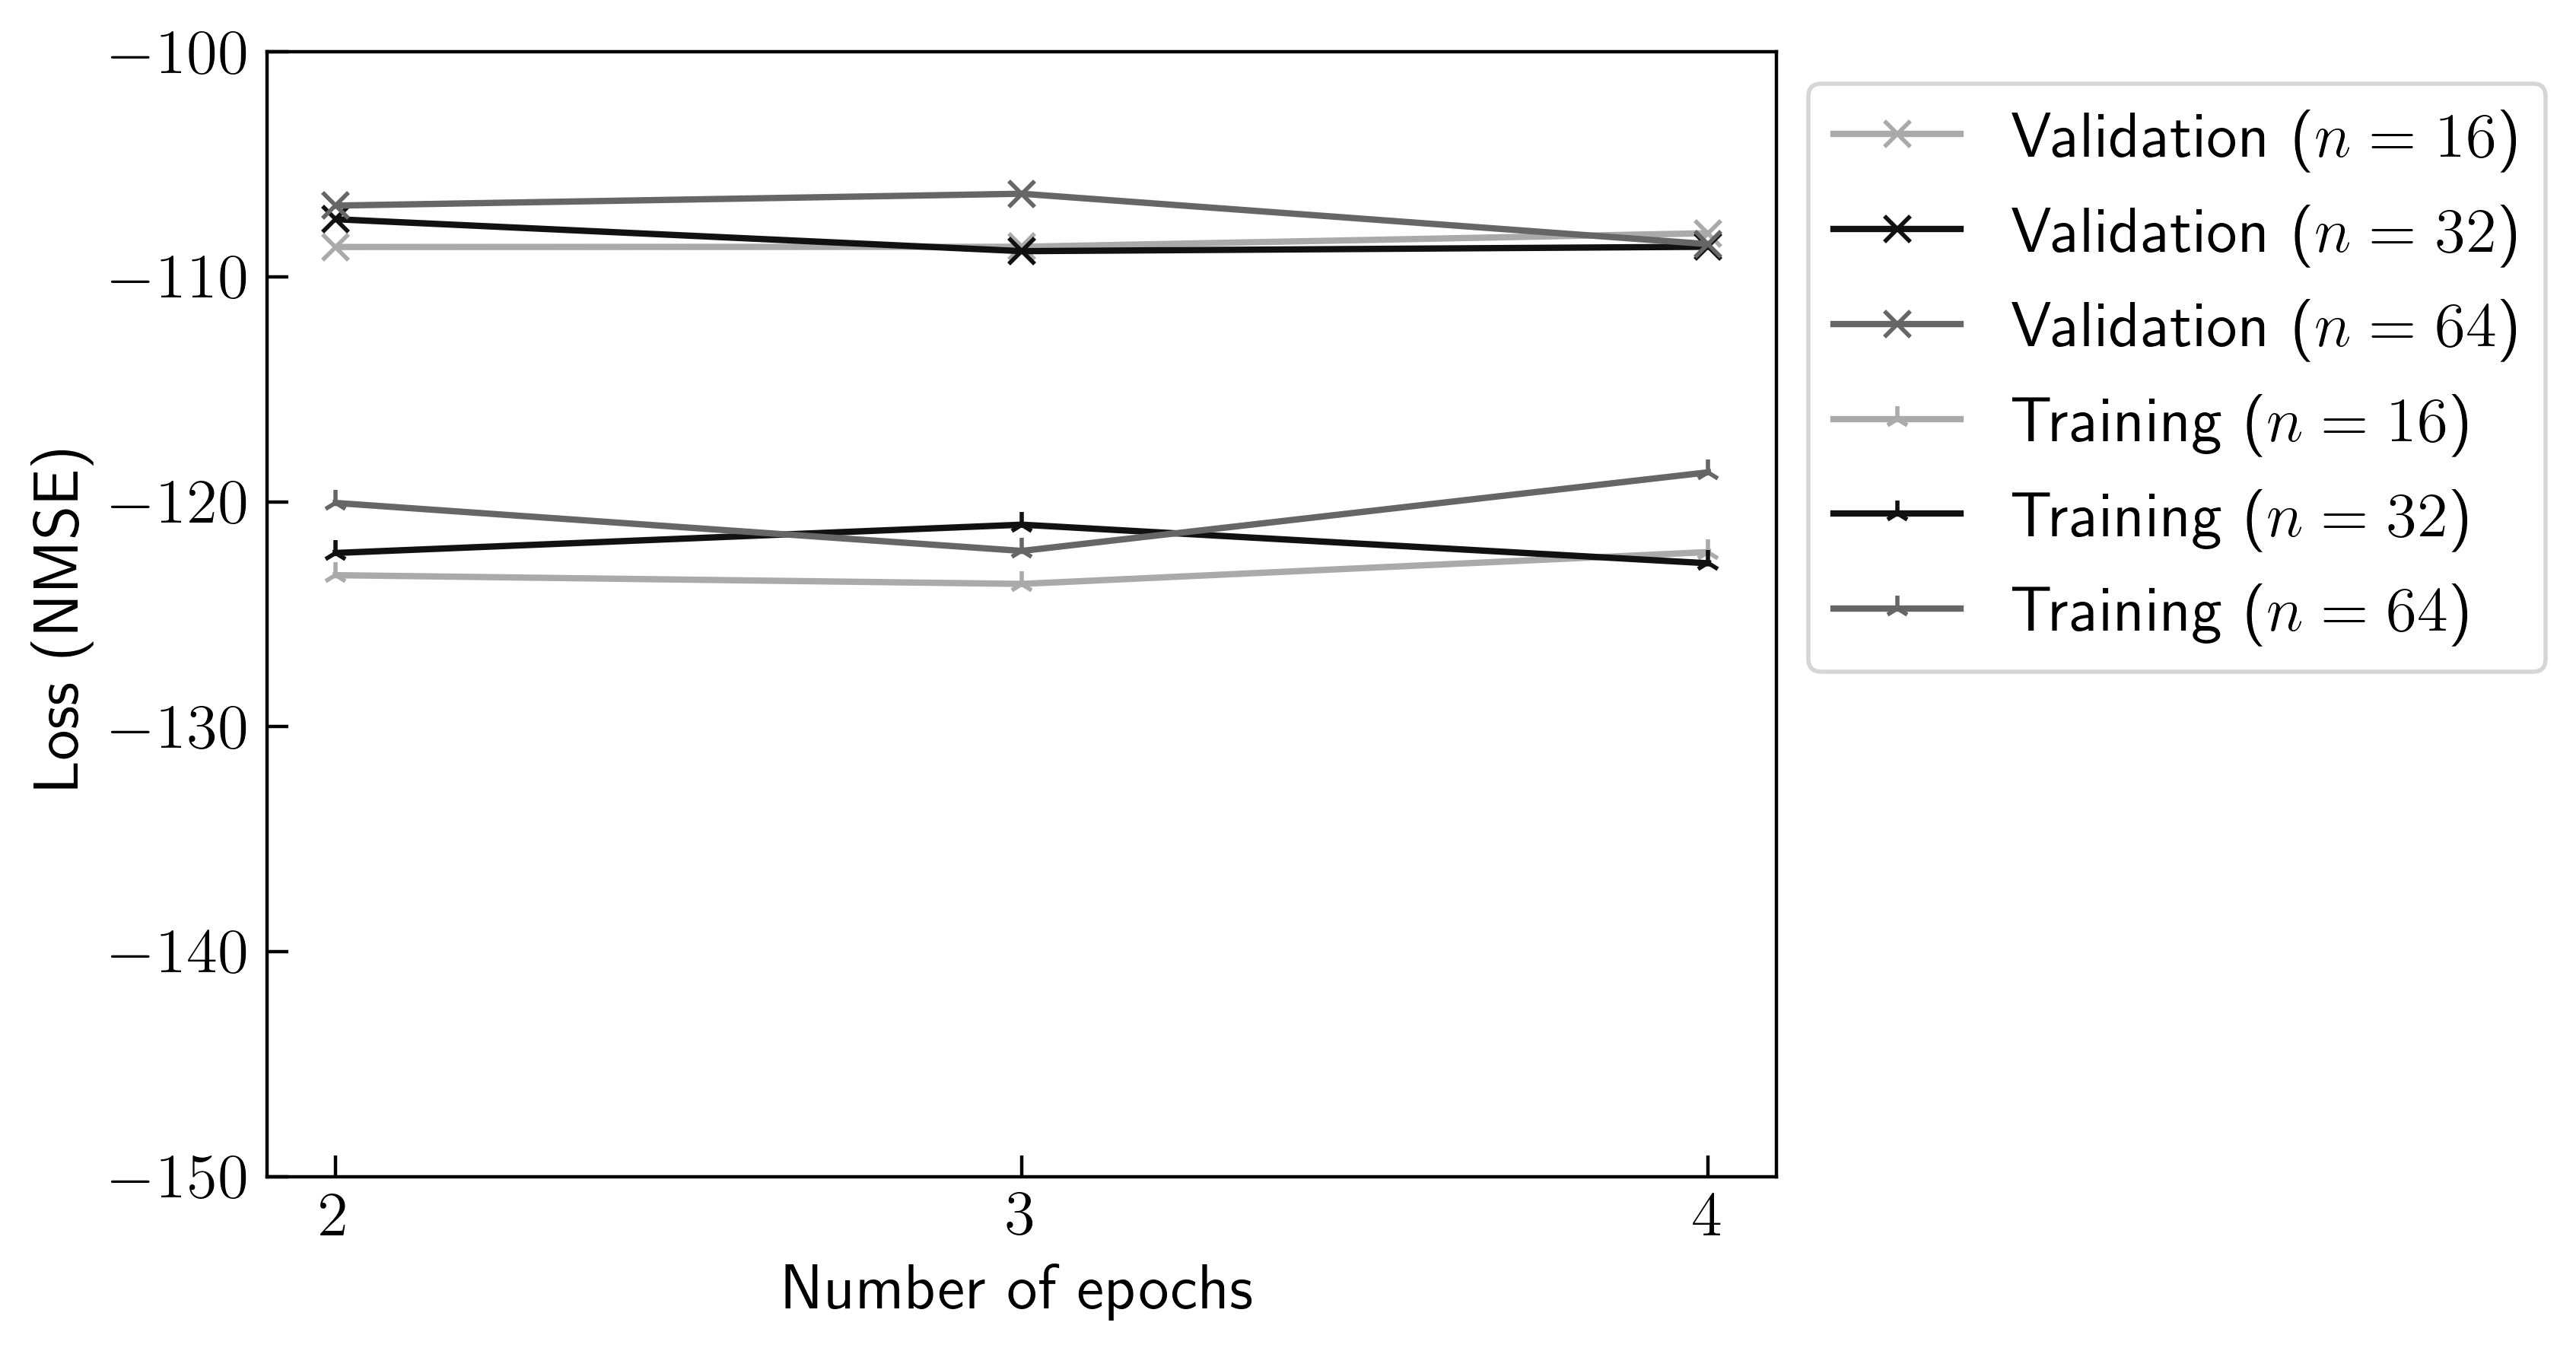
\includegraphics[scale=0.7]{figures/05_impl/01_rfp/02_votes/plot_hyperparams_bert.png}
    \caption{BERT hyperparameter tuning results for review votes ($n$ is batch size).}
    \label{fig:DI_RF_Votes_BERTHP}
\end{figure}

Interestingly, based on these results, it seems that the trained models might be underfitting the training data due to the superior performance of the model against the validation set. Regardless, the best results were produced when a batch size of 64 was used. For a batch size of 64, the results for both 2 and 3 training epochs are almost identical and so, in the interest of reducing training time, 2 epochs would appear to be the optimal choice.

\paragraph{Training Procedure}

The same training procedure was used for the prediction of reviews votes as was used for the prediction of review polarity with the only significant difference being the number of dataset samples being considered.

\subsubsection{Other Models}

\paragraph{Data Splitting}

The dataset splitting procedure was identical to the one outlined for the other models in section \ref{sec:DI_RF_Pol}.

\paragraph{Preprocessing}

The numerous preprocessing steps that were applied to the review text when predicting polarity were also applied here. An additional preprocessing step, discussed already in this section, was the use of a robust scaler to map the number of votes down to a limited range while accounting for outliers.

\paragraph{Hyperparameter Tuning}

Optimal hyperparameters were selected for each model based on the results gathered for the \texttt{eng\_any\_any} sample. The review text was, again, converted into sets of $n$-grams of varying sizes and ranges. For the SGD and ridge regressors, the $\alpha$ parameter was varied. For the LSVR, the $C$ parameter was varied. The methodology used to select parameter ranges, to provide varied results to better identify optimal values, was again applied. The parameter values that were considered can be seen in Table \ref{tab:DI_RF_Votes_BaseHP}.

\begin{table}[ht]
    \centering
    \begin{tabular}{l l l}
        \toprule
        \textbf{Model} & \textbf{Hyperparameter} & \textbf{Values}\\\midrule
        All & $n$-gram range & $(1, 2), (1, 3), (1, 4)$\\
        Ridge & $\alpha$ & $0.01, 0.1, 1, 10$\\
        SGD & $\alpha$ & $10^{-3}, 10^{-4}, 10^{-5}, 10^{-6}$\\
        LSVR & $C$ & $0.01, 0.1, 1, 10$\\
        \bottomrule\\
    \end{tabular}
    \caption{Other model hyperparameters for review votes.}
    \label{tab:DI_RF_Votes_BaseHP}
\end{table}

Two baseline regressors were also used for comparison: one which predicted the mean number of scaled votes and one which predicted the median number of scaled votes. The mean cross-validation NMSE losses, along with the standard deviations, can be seen in Figure \ref{fig:DI_RF_Votes_BaseHP}. In order to improve the clarity of the plots in Figure \ref{fig:DI_RF_Votes_BaseHP}, some results have been offset slightly on the x-axis.

\begin{figure}[ht]
    \hspace*{-0.3in}
    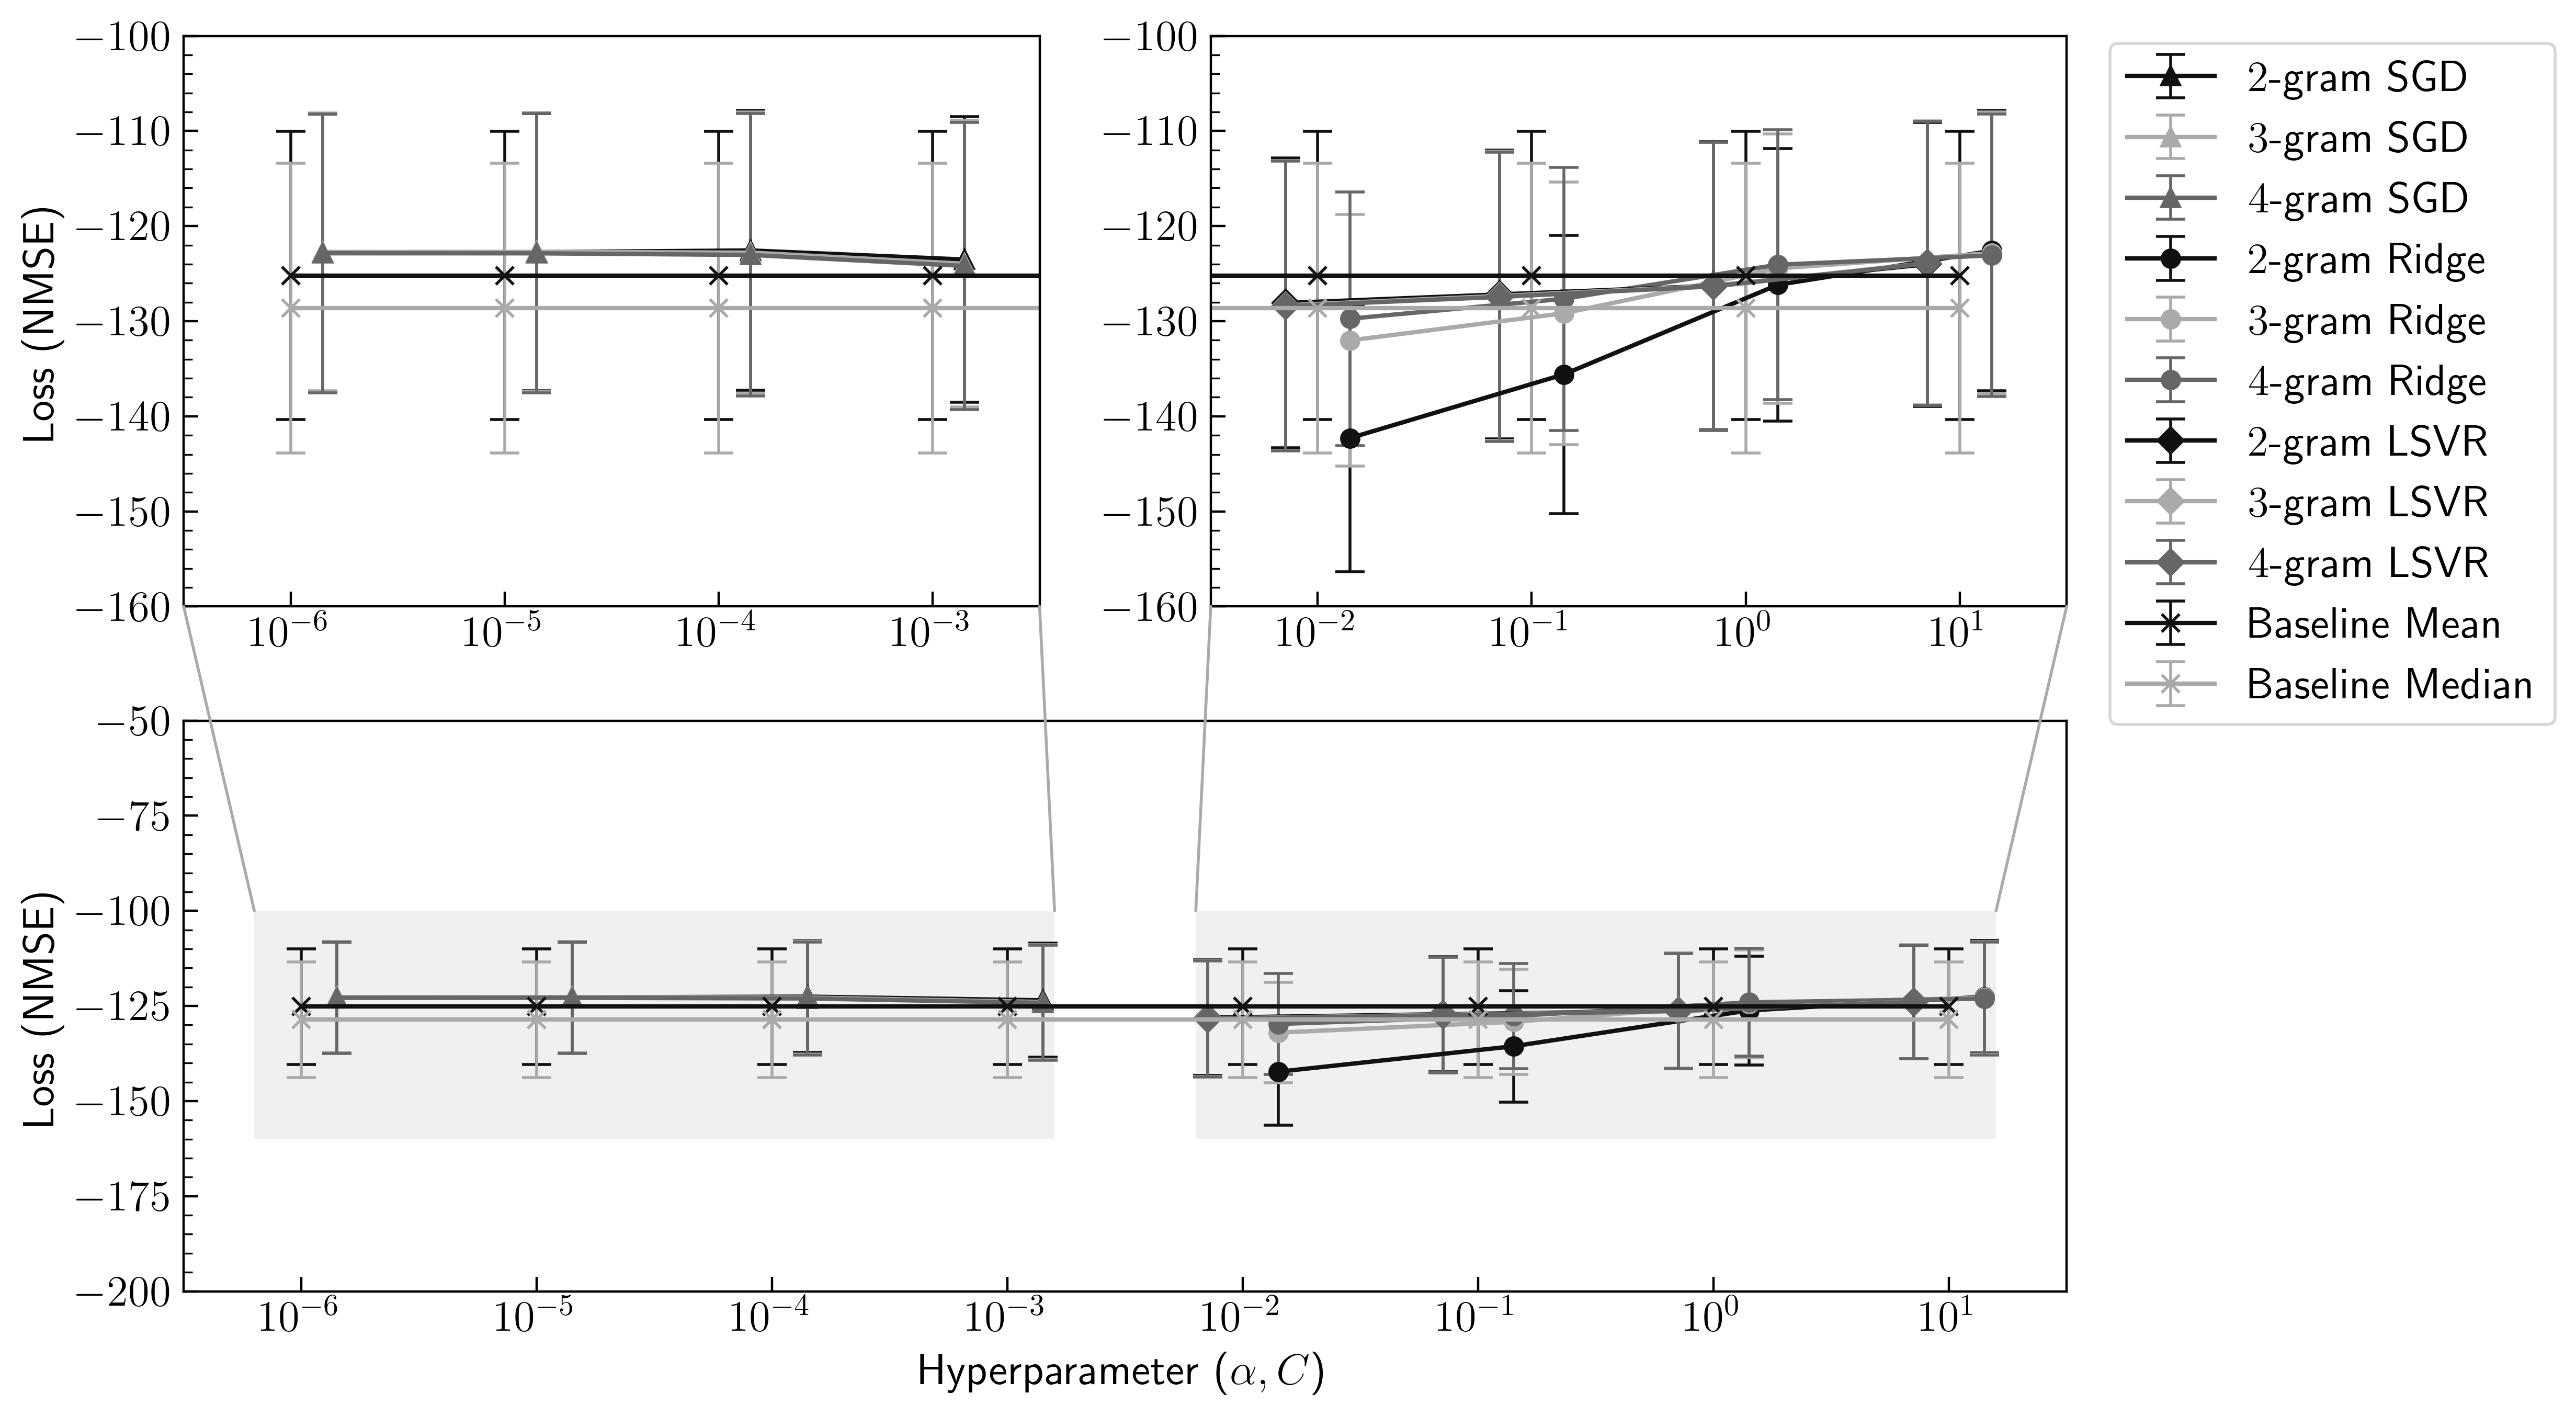
\includegraphics[scale=0.55]{figures/05_impl/01_rfp/02_votes/plot_hyperparams_base.png}
    \caption{Other model hyperparameter tuning results for review votes.}
    \label{fig:DI_RF_Votes_BaseHP}
\end{figure}

The standard deviations of the NMSE losses for each model, despite being quite large, are almost identical and, as such, do not play an important role in determining the optimal choices of hyperparameters.

For the SGD regressor, it would appear that a parameter value of $\alpha=10^{-4}$ with an $n$-gram range of $(1, 2)$ is the best choice; although, no combination of parameters appeared to perform particularly well. For the ridge regressor the optimal choice is slightly more obvious: a parameter value of $\alpha=10$ with an $n$-gram range of $(1, 2)$ produced the best results. For the LSVR, a parameter value of $\alpha=10$ also produces the best results. An $n$-gram range of $(1, 3)$ produced slightly better results than the other ranges, although this is not clear from the plots alone.

\paragraph{Training Procedure}

Each of the optimal regressors was trained and tested on the 6 imbalanced dataset samples. The test results will be discussed in section \ref{sec:Res_RF_Votes}.

\subsection{Playtime} \label{sec:DI_RF_PT}

The process of training the machine learning models to predict the amount of time reviewers spent playing the games they reviewed was almost identical to the process used to predict the number of helpfulness votes reviews received.

The data splitting, preprocessing\footnote{A robust scaler was also applied to the playtime values due to a similar presence of outliers.} and training procedure steps involved in the prediction of review playtime, regardless of the model being trained, are identical to the steps given in section \ref{sec:DI_RF_Votes} concerning the prediction of review votes. As such, they have been excluded.

\subsubsection{BERT}

\paragraph{Hyperparameter Tuning}

Optimal training parameters were, again, selected based on the results gathered for the \texttt{eng\_any\_any} sample. Identical combinations of batch size and training epochs were tested and can be seen, once again, in Table \ref{tab:DI_RF_PT_BERTHP}.

\begin{table}[ht]
    \centering
    \begin{tabular}{l l}
        \toprule
        \textbf{Hyperparameter} & \textbf{Values}\\\midrule
        Batch size & $16, 32, 64$\\
        Epochs & $2, 3, 4$\\
        \bottomrule\\
    \end{tabular}
    \caption{BERT hyperparameters for review playtime.}
    \label{tab:DI_RF_PT_BERTHP}
\end{table}

The NMSE loss for both the training and validation sets can be seen in Figure \ref{fig:DI_RF_PT_BERTHP}.

\begin{figure}[ht]
    \centering
    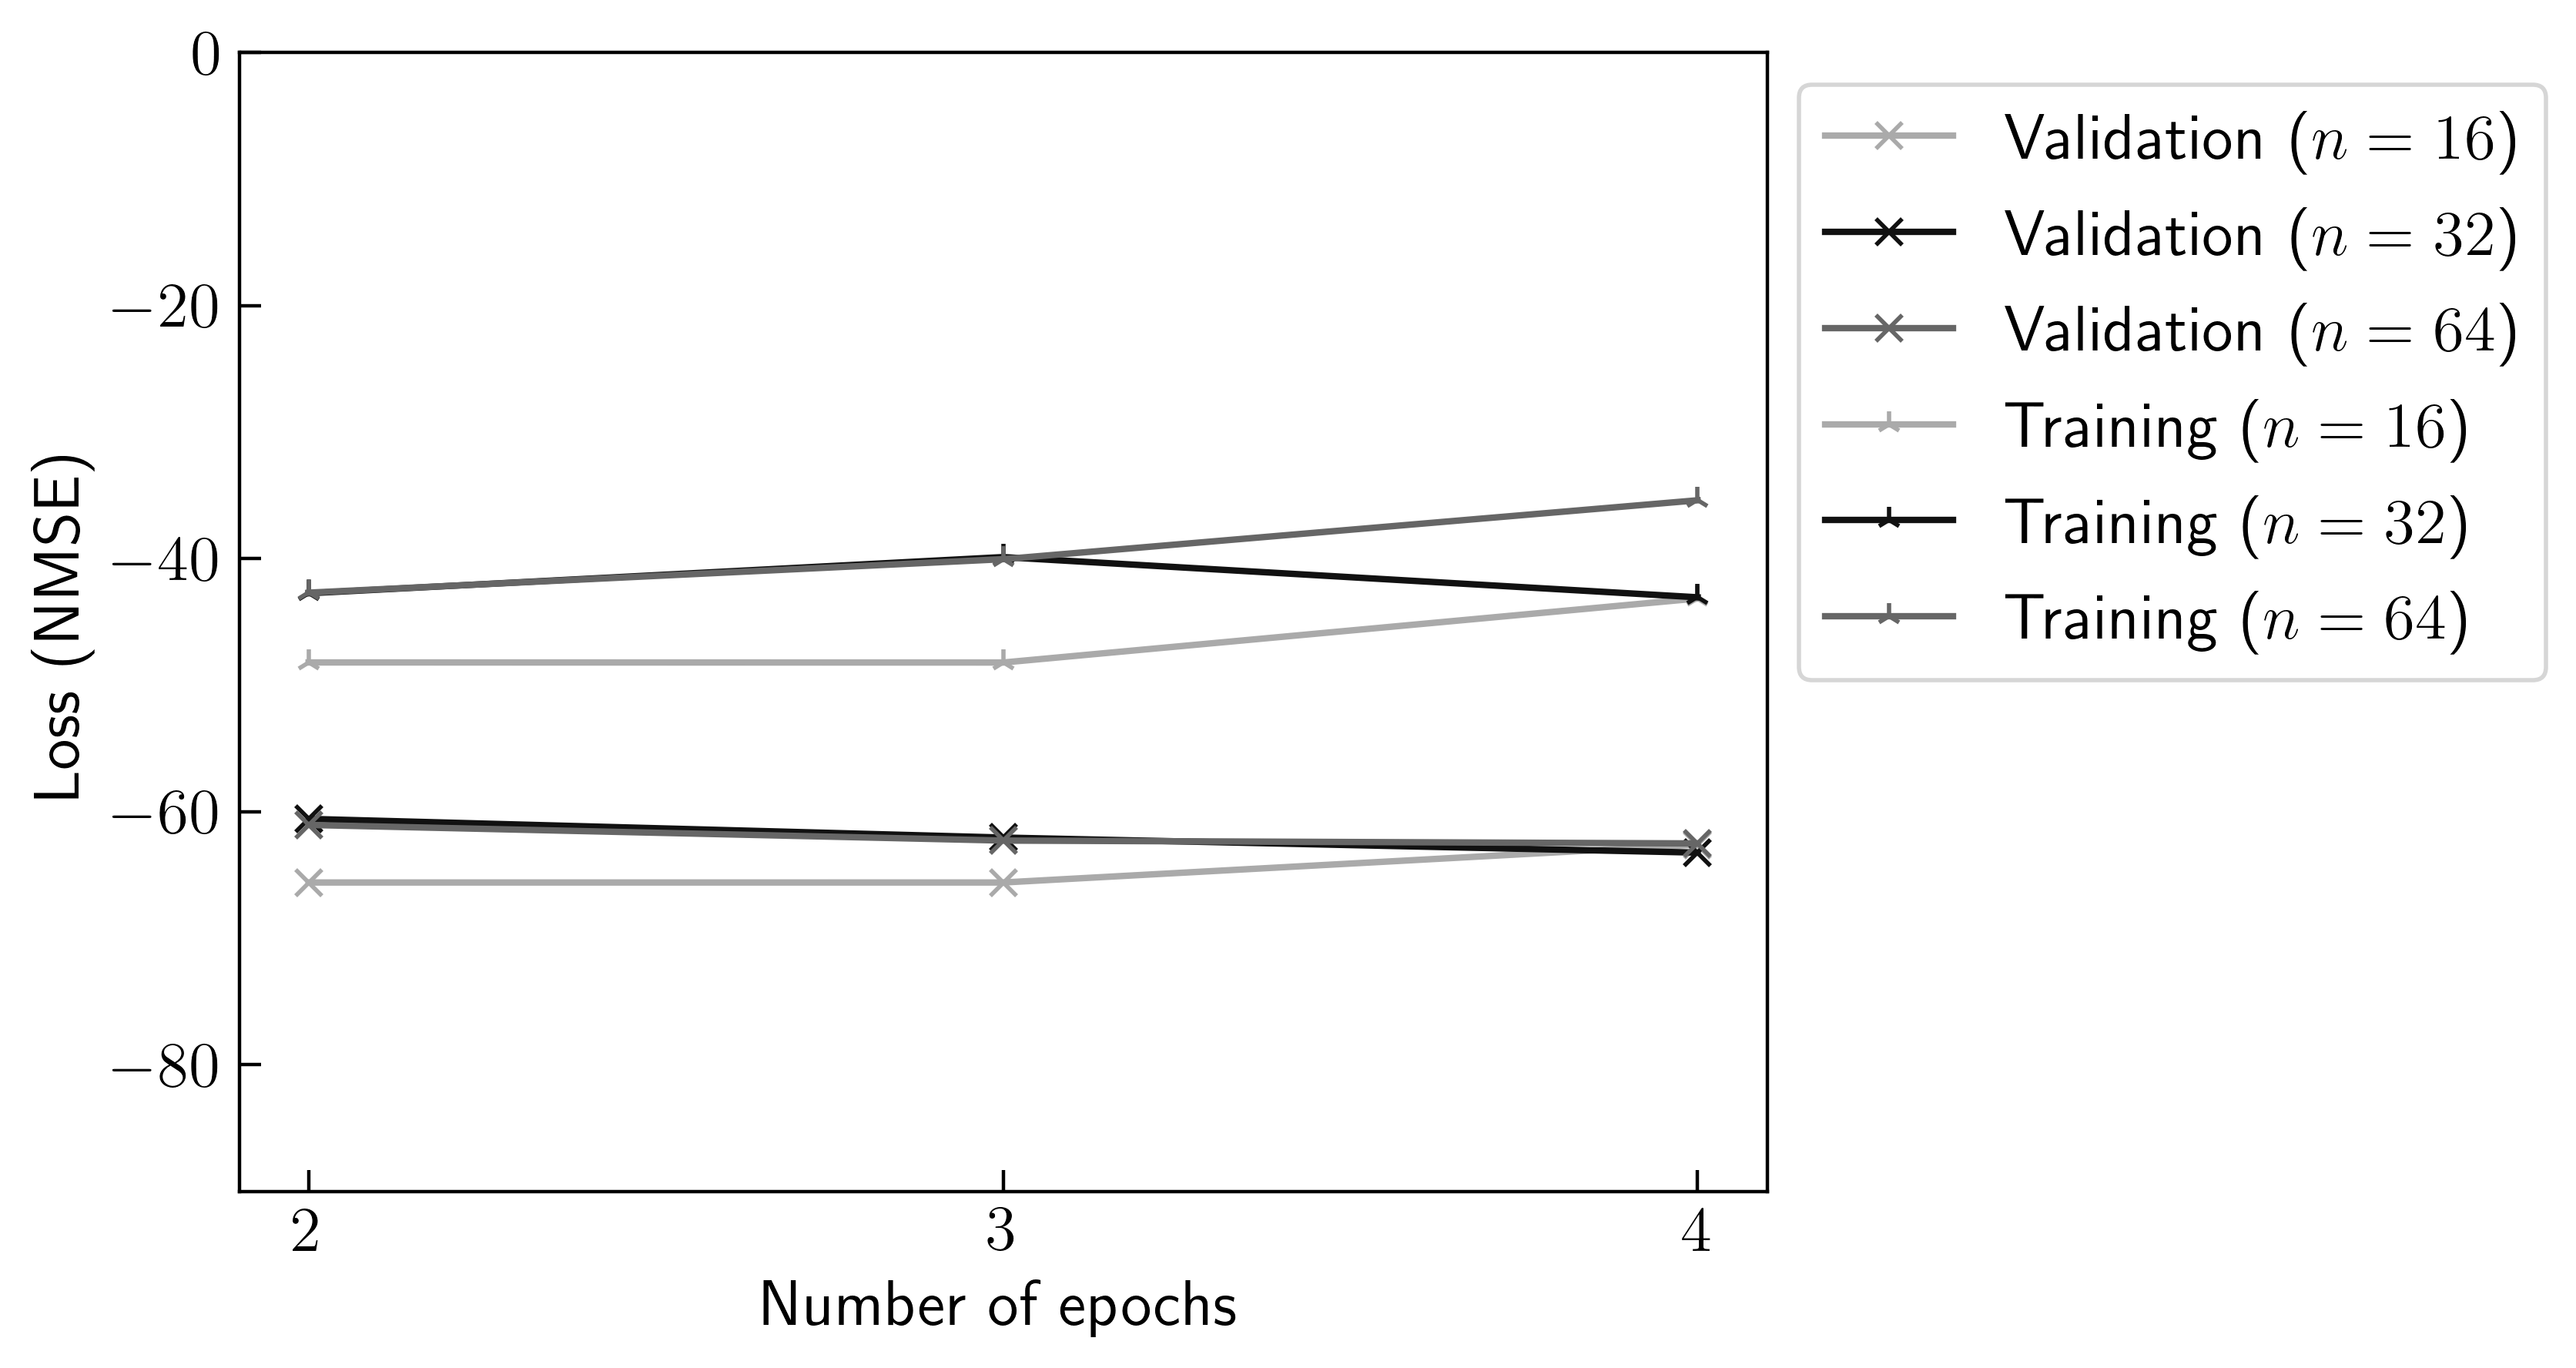
\includegraphics[scale=0.7]{figures/05_impl/01_rfp/03_pt/plot_hyperparams_bert.png}
    \caption{BERT hyperparameter tuning results for review playtime ($n$ is batch size).}
    \label{fig:DI_RF_PT_BERTHP}
\end{figure}

It is quite clear from these results that the optimal choice hyperparameters are batch sizes of 32 or 64 in combination with 2 training epochs, with a batch size of 32 having a slightly better performance\footnote{Due to an initial misreading of the results, a batch size of 64 was chosen when training and testing BERT on the other dataset samples; however, since the NMSE losses for the batch size choices of 32 and 64 were almost identical, this misreading is unlikely to have a significant effect on the overall results.}.

\subsubsection{Other Models}

\paragraph{Hyperparameter Tuning}

The models, hyperparameters and parameter values that were used in the prediction of review votes were also used in the prediction of review playtime. These values can be seen in Table \ref{tab:DI_RF_PT_BaseHP}.

\begin{table}[ht]
    \centering
    \begin{tabular}{l l l}
        \toprule
        \textbf{Model} & \textbf{Hyperparameter} & \textbf{Values}\\\midrule
        All & $n$-gram range & $(1, 2), (1, 3), (1, 4)$\\
        Ridge & $\alpha$ & $0.01, 0.1, 1, 10$\\
        SGD & $\alpha$ & $10^{-3}, 10^{-4}, 10^{-5}, 10^{-6}$\\
        LSVR & $C$ & $0.01, 0.1, 1, 10$\\
        \bottomrule\\
    \end{tabular}
    \caption{Other model hyperparameters for review playtime.}
    \label{tab:DI_RF_PT_BaseHP}
\end{table}

The same two baseline regressors, one that predicted the mean playtime and one that predicted the median playtime, were used for comparison.

The mean cross-validation NMSE losses, along with the standard deviations, can be seen in Figure \ref{fig:DI_RF_PT_BaseHP}. Certain results were, again, offset slightly on the x-axis in order to improve the clarity of the plots.

\begin{figure}[ht]
    \hspace*{-0.3in}
    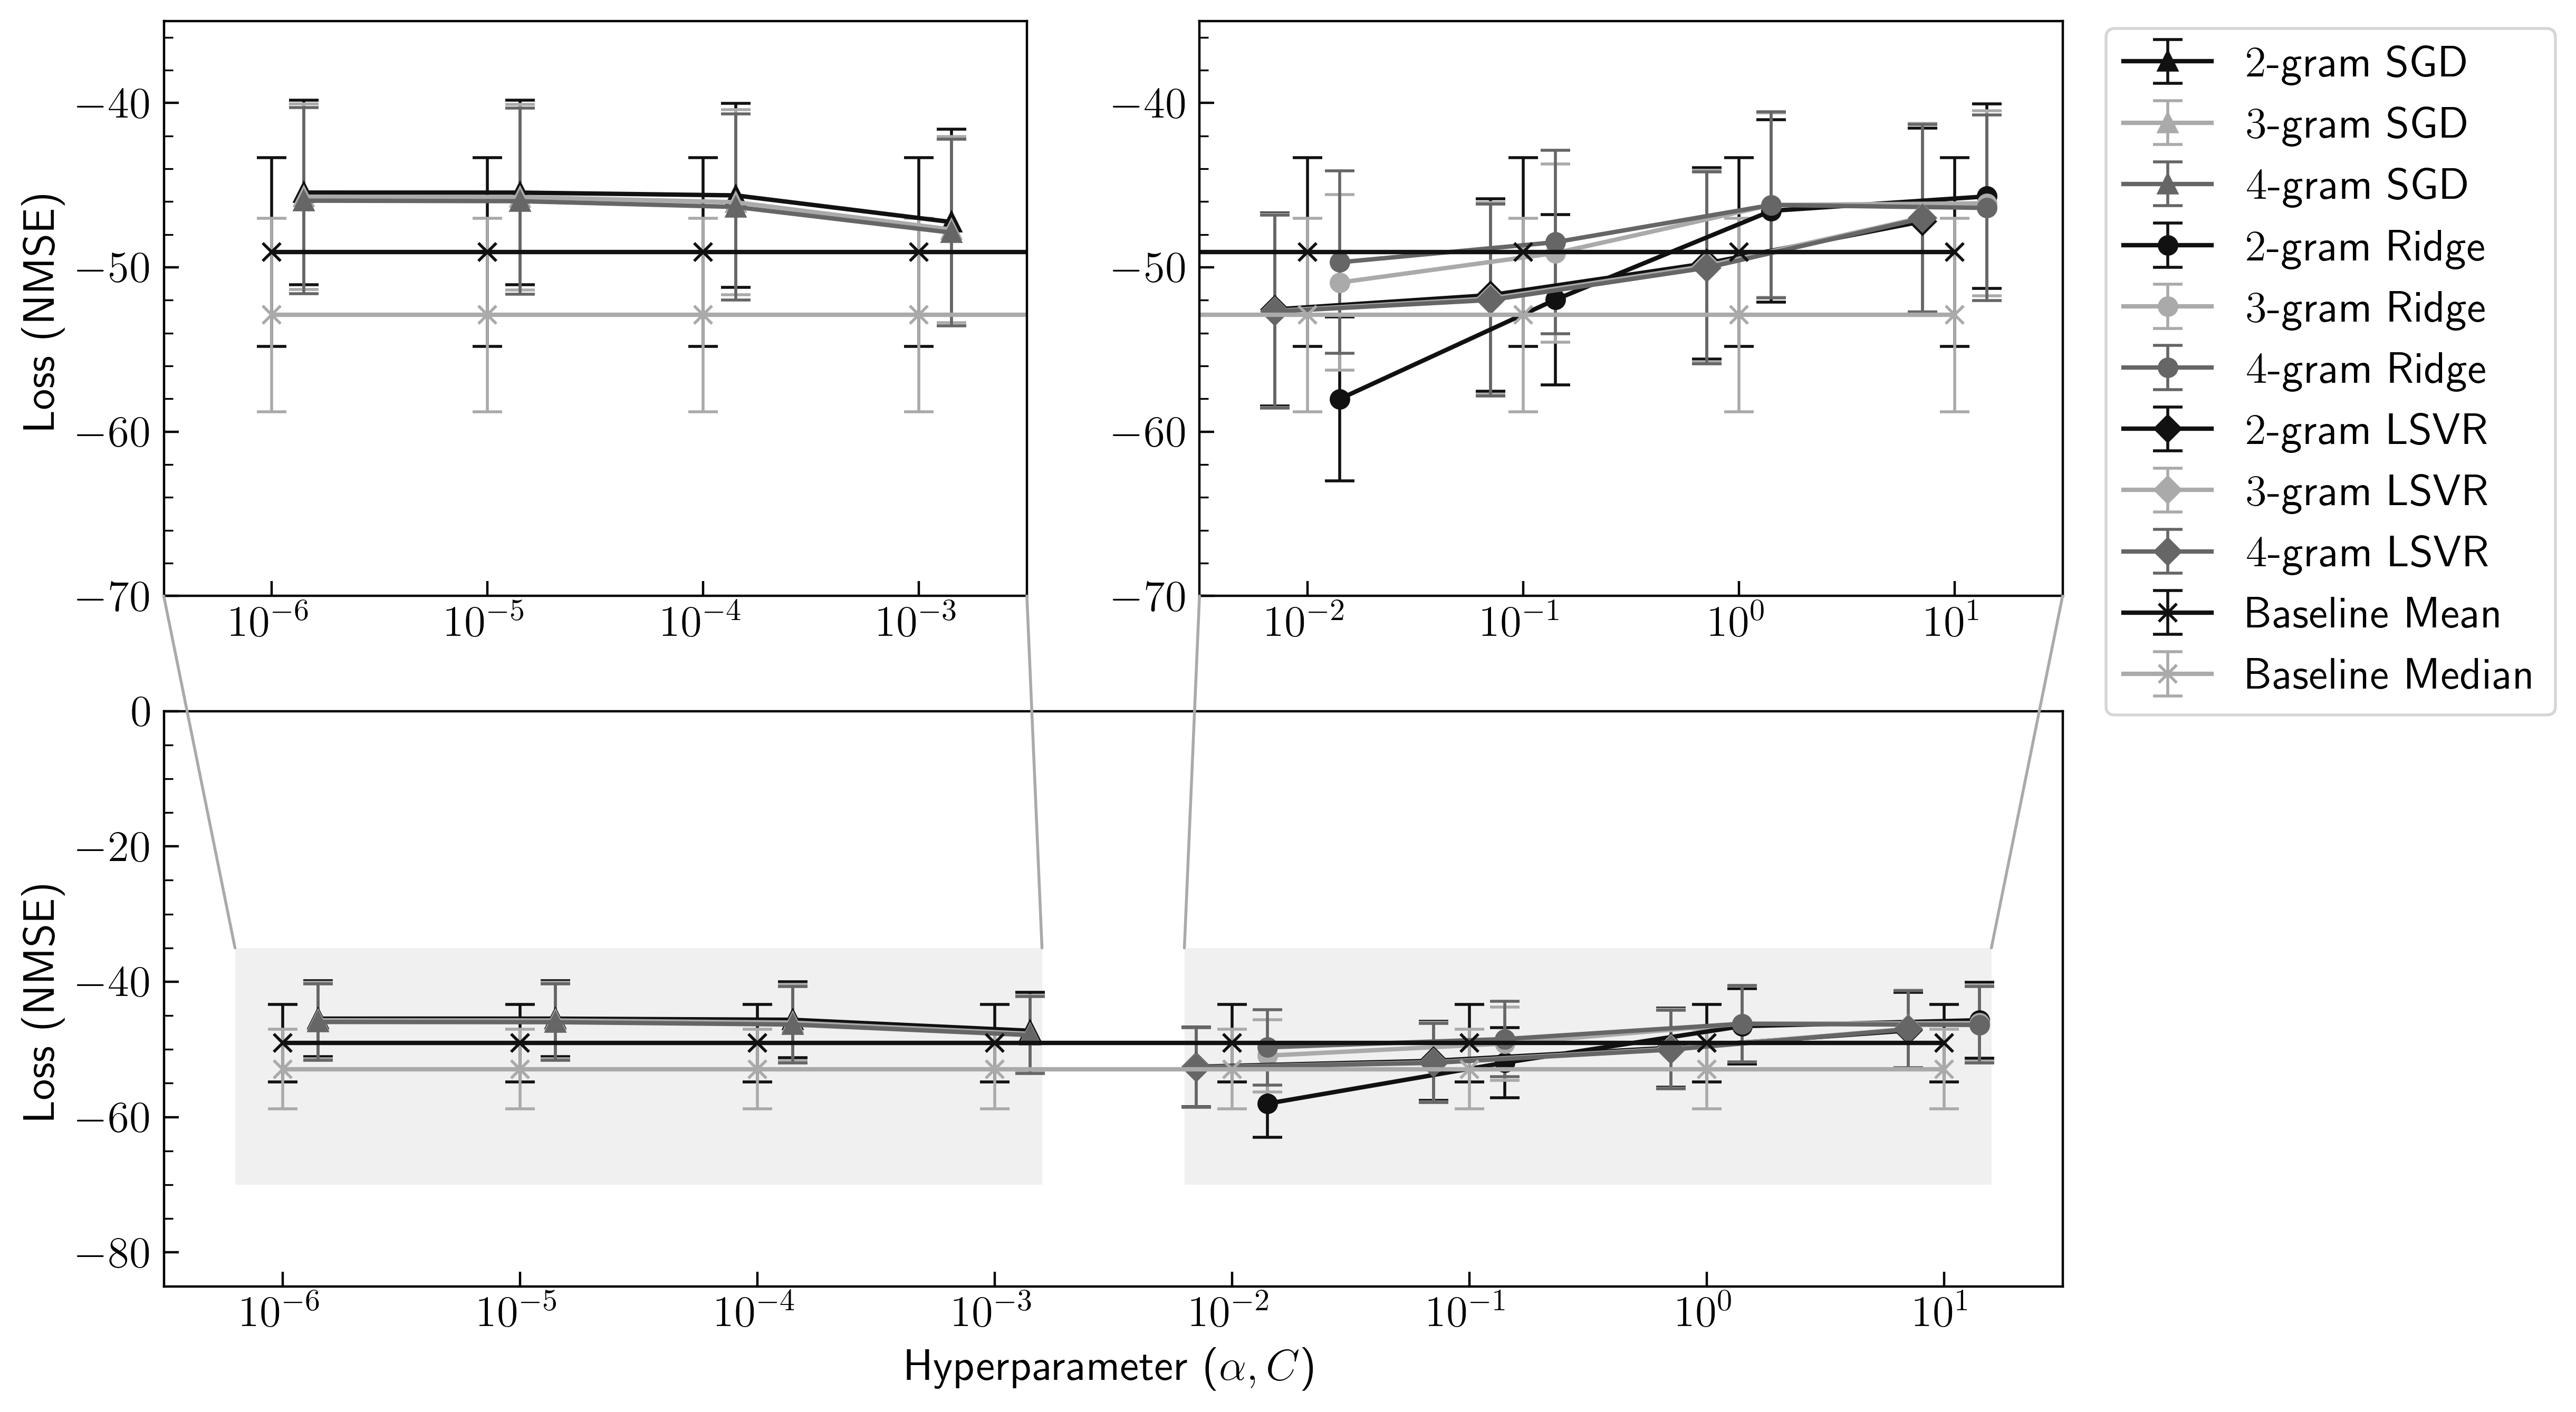
\includegraphics[scale=0.55]{figures/05_impl/01_rfp/03_pt/plot_hyperparams_base.png}
    \caption{Other model hyperparameter tuning results for review playtime.}
    \label{fig:DI_RF_PT_BaseHP}
\end{figure}

The standard deviations of the NMSE losses for each model do not play an important role in the selection of hyperparameters for the same reasons listed in \ref{sec:DI_RF_Votes}.

For the SGD regressor, the $n$-gram range of $(1, 2)$ clearly produces the best results, with the parameter value of $\alpha=10^{-5}$ performing slightly better than the other options. For the ridge regressor, the optimal choices of an $n$-gram range of $(1, 2)$ and a parameter value of $\alpha=10$ are quite clear. For the LSVR, a value of $C=10$ is clearly the optimal choice. Although it isn't clear from the plot, an $n$-gram range of $(1, 3)$ produces the best results when $C=10$.

\section{Representative Users} \label{sec:DI_RU}

Text.

\subsection{Dataset Sampling and Preparation}

Text.

\subsection{BERT}

\subsubsection{Data Splitting and Preprocessing}

Text.

\subsubsection{Hyperparameter Tuning}

Text.

\subsubsection{Training and Testing Procedure}

Text.

\subsection{Other Models}

\subsubsection{Data Splitting and Preprocessing}

Text.

\subsubsection{Hyperparameter Tuning}

Text.

\subsubsection{Training and Testing Procedure}

Text.
